\chapter{LibChain}
\section{Architecture Overview}
The main architecture of LibChain is divided into three parts: React that is used to implement a prototypical library page, NodeJs that provides a REST interface that enables the connection to the frontend and the ethereum blockchain where the LibChain contracts are deployed on. Communication between the NodeJs backend and the blockchain are realized through the \texttt{Web3.js} api.

\vspace{0.3cm}
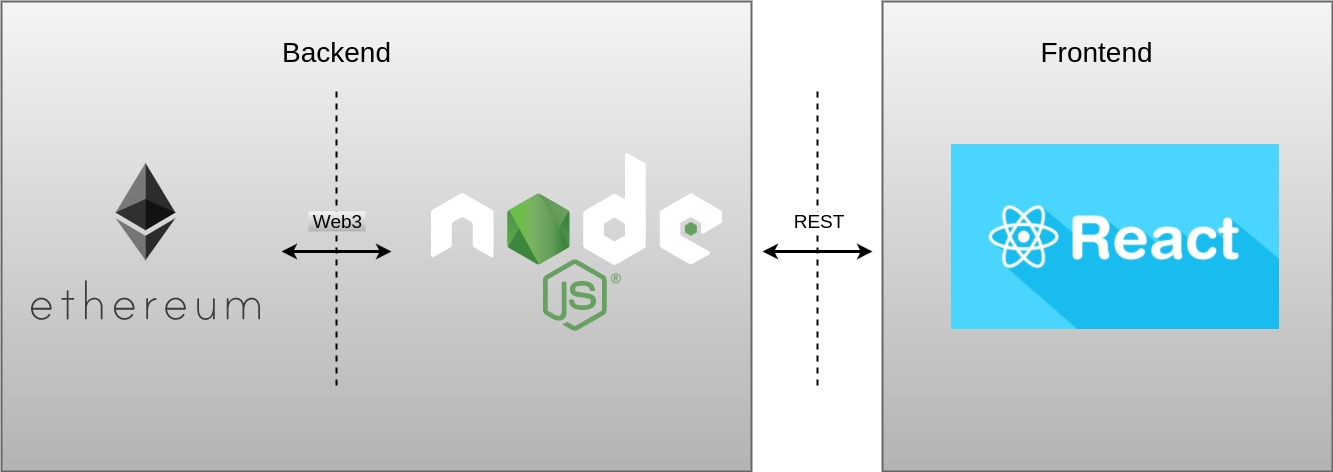
\includegraphics[width=\textwidth]{architecture.jpg}
\subsection{Backend}


\subsection{Frontend}


\section{Smart Contracts}
LibChain implements contracts for publisher, libraries and books that provides functionality to publish, buy and lend books in the LibChain ecosystem.

\vspace{0.3cm}
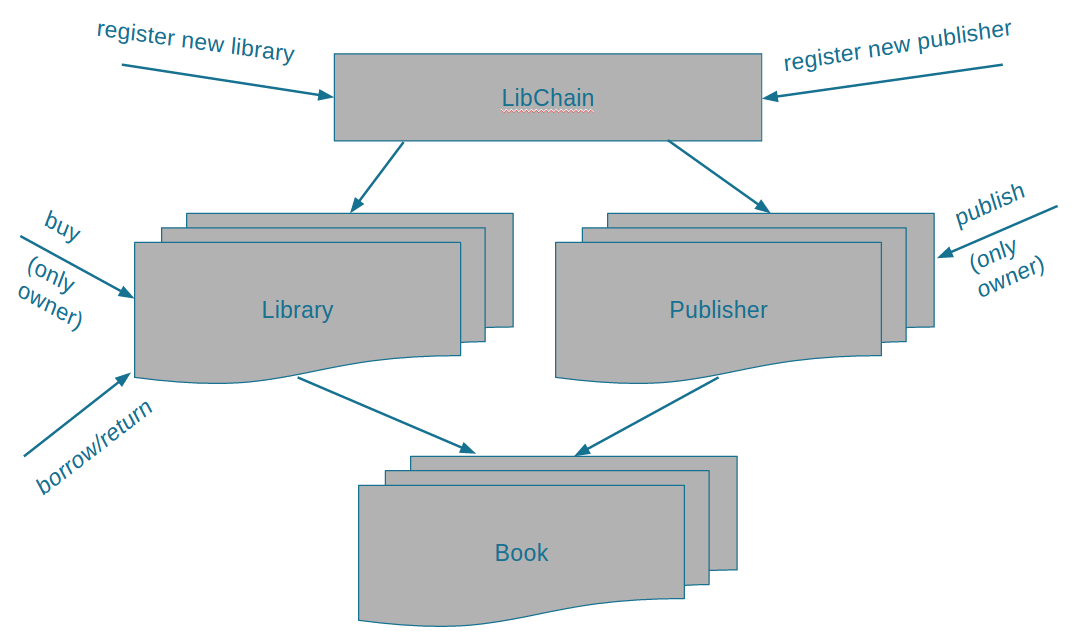
\includegraphics[width=\textwidth]{contracts.png}

\subsection{LibChain}
The LibChain contract collects the available libraries and publisher. It provides functions to create new instances of publishers and libraries.

\subsection{Book}
\begin{lstlisting}
contract Book {

	address public _owner;
	string public _publisher;
	uint public _year;
	string public _gateway;
	string public _isbn;
	
	mapping (address => uint) public _balances;
	uint sumOfSoldInstances;
	uint sumOfLoans;
  
	function Book(string pub, uint year, string id, string gate) {
  	_owner = msg.sender;
		_publisher = pub;
		_year = year;
		_gateway = gate;
		_isbn = id;
	}


	function getBookInfo() constant returns (uint, string, string, 		string, uint, address, address) 
	{
	 	return (_year, _isbn, _gateway, _publisher, 	_balances[msg.sender], _owner, this);
	}

	function buy(address buyer, uint amount) {
		_balances[buyer] += amount;
		sumOfSoldInstances++;
	}

}
\end{lstlisting}

\subsection{Publisher}
The publisher contract allows to instantiate new books and add them to the publishers catalogue.

\begin{lstlisting}
function publishBook(uint year, string id, string gate) returns(address bookContract){
		publishedBooks.push(new Book(name, year, id, gate));
		sumOfPublications++;
		(..)
		return publishedBooks[bookNum-1];
	}
\end{lstlisting}

As a Book is a smart contract, it get's a unique address. Therefore, a Library is able to call the \texttt{buyBook}-function to  



\begin{lstlisting}
	function buyBook(address bookContract, uint amount) constant {
		Book book = Book(bookContract);
		book.buy(msg.sender, amount);	
		bills[msg.sender][bookContract] += amount;

		sumOfSoldInstances += amount;
	}
\end{lstlisting}

\subsection{Library}
\begin{lstlisting}
	function buy(address bookContract, address publisherContract, uint amount) returns (bool) {
		Publisher pub = Publisher(publisherContract);
		pub.buyBook(bookContract, amount);
        Book book = Book(bookContract);
        if(inventory[book].amount == 0){
            inventory[book] = BookMeta(book, amount, amount);
		    _libBooks.push(book);
		} else {
            inventory[book].amount += amount;
            inventory[book].availableInstances += amount;
		}

		sumOfBoughtInstances += amount;
		return true;
	}
\end{lstlisting}

\begin{lstlisting}
	    function hasAccessToInstance(string userId, string pubkey, address bookAddress) constant returns (uint) {
        if(sha3(pubkey) == sha3("")) return 0;

        if(sha3(users[userId].pubkeys[bookAddress]) == sha3(pubkey)){
            // has access
            return 1;
        }

        // no access
        return 0;
    }
\end{lstlisting}



\begin{lstlisting}
function borrow(address bookContract, string publicKey, string userId) returns (bool) {

		if(inventory[bookContract].availableInstances <= 0) return false;

		//check if this book already loaned to user
        if (sha3(users[userId].pubkeys[bookContract]) != sha3("")){
            return false;
        }


		Book book = Book(bookContract);
        for (var i = 0; i < inventory[bookContract].amount; i++) {
            if (sha3(inventory[bookContract].pubkeys[i]) == sha3("")) {
                inventory[bookContract].pubkeys[i] = publicKey;
                inventory[bookContract].availableInstances--;

                // store loan to user object
                users[userId].loanedBooks.push(bookContract);
                users[userId].pubkeys[bookContract] = publicKey;

                book.borrow(msg.sender);
                sumOfLoans++;

                return true;
            }
        }

        return false;
	}
\end{lstlisting}


\begin{lstlisting}
	function returnBook(address bookContract, string publicKey, string userId) returns (bool) {
    		if(inventory[bookContract].amount <= 0) return false;
    		Book book = Book(bookContract);
            for (var i = 0; i < inventory[bookContract].amount; i++) {
                if (sha3(inventory[bookContract].pubkeys[i]) == sha3(publicKey)) {
                    inventory[bookContract].pubkeys[i] = "";
                    inventory[bookContract].availableInstances++;


                    // remove book from user object
                    for (var j = 0; j < users[userId].loanedBooks.length; j++) {
                        if(users[userId].loanedBooks[i] == bookContract){
                            delete users[userId].loanedBooks[j];
                            break;
                        }
                    }
                    users[userId].pubkeys[bookContract] = "";
                    sumOfReturns;
                    return true;
                }
            }

        return false;
    }
\end{lstlisting}

%\begin{itemize}
%\item buying books
%\item lending books
%\item provide confirmation methods for publishers, wheter a user has acces or not
%\end{itemize}



\section{Use Cases}
%\begin{itemize}
%\item short overview of use cases
%\end{itemize}
\subsection{Book-Purchase}

\vspace{0.3cm}
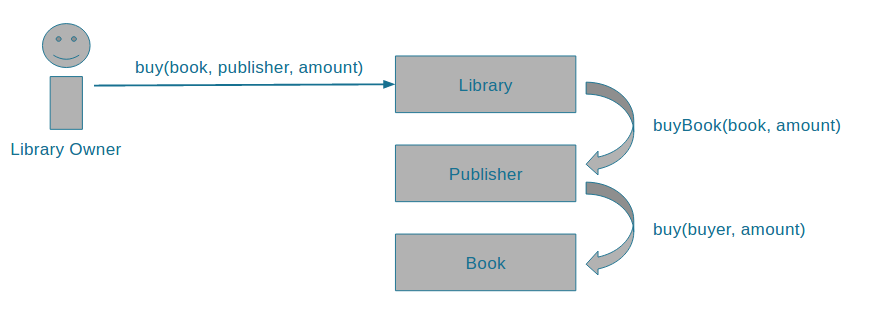
\includegraphics[width=\textwidth]{purchase.png}
%\begin{itemize}
%\item a library want's to buy some book instances
%\item calling the buy method on library contract
%\end{itemize}
\subsection{Book-Borrow}
\vspace{0.3cm}
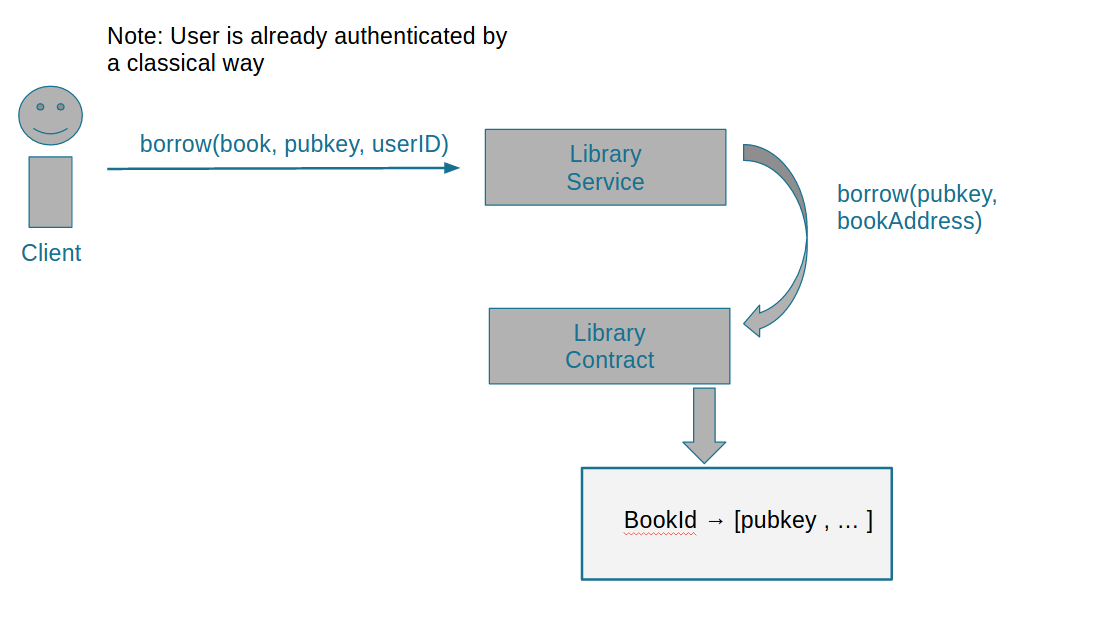
\includegraphics[width=\textwidth]{borrow.png}


\subsection{Access to digital media}
\vspace{0.3cm}
\includegraphics[width=\textwidth]{access.png}


\subsection{Book-Return}

\section{Metrics}

\section{How to implement a Publisher Service?}

